\subsection{Limma-Voom}

Limma-Voom is a method applied in order to perform DE analysis on RNA-seq data.
It estimates the mean-variance relationship of the log-counts, generates a precision weight for each observation and enters these into the limma empirical Bayes analysis pipeline.

The read-counts are first log-cpm transformed (Formula \ref{formula:logcpm}) as a means of normalizing the data.
However, the probability distribution for counts are naturally heteroscedastic, with larger variances for larger counts.
\textit{Law et al.} conclude that the log-cpm values generally show a smoothly decreasing mean-variance trend with count size, and that the log-cpm transformation roughly de-trends the variance as a function of count size for genes with higher counts.

\begin{equation}
    log_2CPM = log2\left(\frac{count * 10^6}{\sum_{j=1}^{N} count_j}\right)
    \label{formula:logcpm}
\end{equation}

To analyse the RNA-seq data, the log-cpm values are inputted into the limma software.
However, due to the mean-variance trend in lower counts, there should be a correction applied.
First, gene-wise linear models are fitted using the normalized log-cpm values, taking into account experimental design, treatment conditions, replicates and so on (Formula \ref{formula:limma_model}).
The residual standard deviations for each gene is plotted, and modeled on a observation-level in a non-parametric way using a lowess fit as a function of the average log-count (Figure \ref{fig:voom_mean_var_trend}).
Using the fitted log-CPM value for each observation, a predicted count is generated and used to interpolate a predicted standard deviation for that observation.
In the end, the inverse squared predicted standard deviation for each observation, becomes the weight for that observation in that gene model that are now fitted using weighted least squares.

\begin{equation}
    logCPM(gene_j) = \beta_0 + \beta_{1}x_{1} + \cdots + \epsilon 
    \label{formula:limma_model}
\end{equation}

\begin{figure}[t]
    \centering
    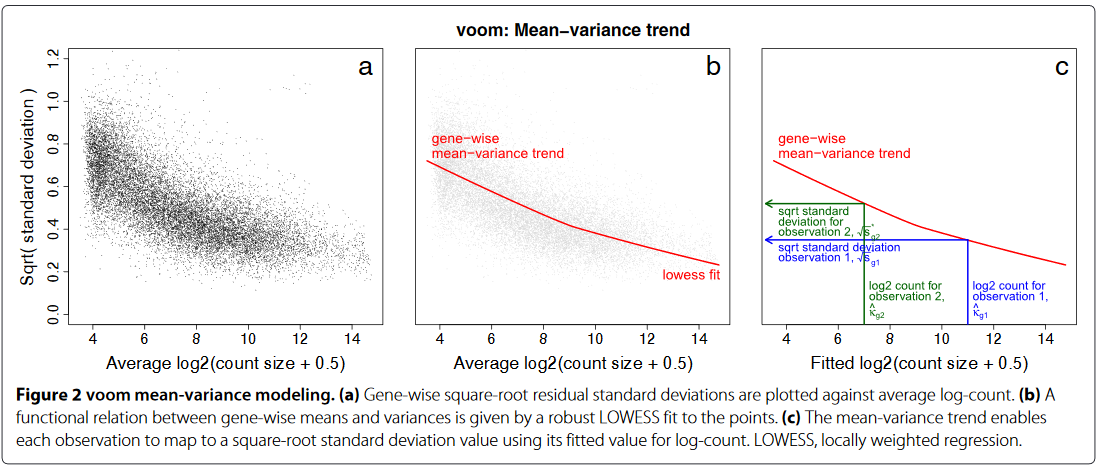
\includegraphics[width=\textwidth]{figs/voom_mean_var_trend.png}
    \label{fig:voom_mean_var_trend}
\end{figure}

This procedure accounts for the systematic relationship between the mean expression level and the residual variance.
However, this does only provide precision-weights that depend on the mean-variance trend and do not stabalize gene-wise variance estimates. 
Some genes may still have highly noisy or extreme variances due to the limited sample sizes, high biological variability or other random effects.
To solve this, the emperical Bayes method comes in.
It targets the residual variance from each gene-wise models by borrowing information across all genes to estimate the pooled prior variance, and shrinks individual gene-wise variances towards this pooled prior.
T- and F-tests can than be performed using this shrinked variance, for which we call them \textit{moderated} tests.

The main take away is that voom corrects for the systematic mean-variance trend across genes and samples, making model fitting more accurate, while eBayes stabalizes the individual gene-wise variance estimates by borrowing strength across genes, which is critical for robust hypothesis testing.